\clearpage
\subsection{Study III --- higher-order angular modes: the $A{=}3$ directional closure}

\paragraph{The angular-convergence difficulty of Study II.}
The results of the preceding paragraphs show that the
rectangular-node model still carries a large eigenvalue bias on the MOX
assembly even at $M{=}24$ ($-98.9$~pcm at $S{=}1$, $-33.5$~pcm at its
best $S{=}2$), and that on every geometry the $M$-convergence is
non-monotonic at low order, flattening only at the highest segment
count. The $S$-response is non-monotonic as well: on the MOX row a
single subdivision buys the best point and any further subdivision
degrades it again. Neither knob can be pushed to convergence in the old
closure. The diagnosis is that the original PSN carries \emph{one}
angular unknown per azimuthal segment: the intra-segment angular
distribution is averaged into a single coefficient, and for a geometry
with strong fuel--water coupling --- where the angular flux varies
sharply across a $7.5^{\circ}$ segment as directions move from
fuel-grazing to water streaming --- that single mode carries a
representation error that segment subdivision $M$ and spatial
subdivision $S$ dilute but do not remove within the range of this work
(Study II: a $-99$~pcm MOX bias persisting to $M{=}24$).

\subsubsection{The $A{=}3$ directional closure, derived from the PSN formulation}

\emph{Where the original PSN approximates.}
Start from the steady multi-group transport equation inside a
homogeneous node of the original phase-space nodal method~\cite{psn2027},
Eq.~(2.1a) of that paper:
\begin{equation}
\boldsymbol{\Omega}\cdot\nabla\psi(\boldsymbol{\Omega},\mathbf{r})
+\Sigma_t\psi(\boldsymbol{\Omega},\mathbf{r}) = \frac{Q(\mathbf{r})}{4\pi},
\label{eq:transport}
\end{equation}
with $Q$ the isotropic (scattering $+$ fission) source and
$\phi=\int\psi\,d\Omega$. The lowest GSPN ansatz, Eq.~(2.3a) of
Ref.~\cite{psn2027},
\begin{equation}
\psi_{P_1} = \frac{1}{4\pi}\Big[\phi_0
-\frac{1}{\Sigma_t}\boldsymbol{\Omega}\cdot\nabla\phi_0\Big],
\end{equation}
annihilates the first-derivative term when substituted back into
Eq.~\eqref{eq:transport}, leaving
$-\frac{1}{\Sigma_t}(\boldsymbol{\Omega}\cdot\nabla)^2\phi_0
+\Sigma_t\phi_0 = Q$, which no single angle-independent
$\phi_0$ can satisfy for every direction. The original paper therefore
integrates over the full solid angle, using
$\langle\Omega_j\Omega_l\rangle_{4\pi}=\delta_{jl}/3$, and obtains the
isotropic diffusion equation, its Eq.~(2.3c),
\begin{equation}
-\frac{1}{3\Sigma_t}\nabla^2\phi_0+\Sigma_t\phi_0 = Q,
\label{eq:diff3c}
\end{equation}
whose wave number is $k^2 = 3\Sigma_t^2$ (Eq.~(2.11b)). The reconstruction
$\psi = \frac{1}{4\pi}[\phi - \Sigma_t^{-1}\boldsymbol{\Omega}\cdot\nabla\phi]$
with $\phi=\phi_0+C$ (Eqs.~(2.3d,e)) adds one node-constant degree of
freedom fixed by the phase-space node balance (Eq.~(2.9a)), but the
\emph{body} of the node is still governed by the full-solid-angle
average of Eq.~\eqref{eq:diff3c}: the direction-dependent operator
$(\boldsymbol{\Omega}\cdot\nabla)^2$ has been replaced by the
angle-averaged Laplacian. The face quantities, by contrast, retain the
true angular second moments: the original face current
(Eq.~(2.8b)) carries the polar factor
$\beta_i/3=\tau_i/2$ with $\beta_i=\tfrac32\,\tau_i$
(Eq.~(2.8d)) and the azimuthal
chordal-averaging factor $\gamma_m=\sin\Delta\varphi_m/\Delta\varphi_m$,
i.e.\\ a direction-dependent diffusion tensor, with
$c_m$ the segment centre,
\[
D^{(0)}_{im} = \frac{\tau_i}{2\Sigma_t}
\begin{pmatrix}
1+\gamma_m\cos 2c_m & \gamma_m\sin 2c_m\\
\gamma_m\sin 2c_m & 1-\gamma_m\cos 2c_m
\end{pmatrix}
\]
with $\tau_i=\langle\sin^2\theta\rangle_i$.
\textbf{The original
method thus evaluates the body on the isotropic scale while the faces
carry the anisotropic angular moments; the $A{=}3$ directional closure
makes the body use the same angular second moments as the faces, at
every angular order.}

\emph{Parity elimination and the exact even-parity equation.}
Write $f=4\pi\psi$ and split into even and odd parity,
$e(\Omega)=\tfrac12[f(\Omega)+f(-\Omega)]$,
$o(\Omega)=\tfrac12[f(\Omega)-f(-\Omega)]$:
$\boldsymbol{\Omega}\cdot\nabla o+\Sigma_t e=Q$ and
$\boldsymbol{\Omega}\cdot\nabla e+\Sigma_t o=0$. Inside a node of
constant $\Sigma_t$ the odd parity is eliminated \emph{exactly},
$o=-\Sigma_t^{-1}\boldsymbol{\Omega}\cdot\nabla e$, giving the
directional second-order equation
\begin{equation}
-\boldsymbol{\Omega}\cdot\nabla\Big(\Sigma_t^{-1}
\boldsymbol{\Omega}\cdot\nabla e\Big)+\Sigma_t e = Q.
\label{eq:A1}
\end{equation}
This is the mother equation of the closure. If the even-parity trial
field is restricted to be angle-independent and
Eq.~\eqref{eq:A1} is then averaged over the full solid angle,
$\langle\boldsymbol{\Omega}\boldsymbol{\Omega}\rangle_{4\pi}
=\tfrac13\mathbf{I}$, the result is Eq.~\eqref{eq:diff3c}, and the
original reconstruction (2.3a) is recovered as the exact
parity-elimination identity. The projection order matters: the even parity is projected
\emph{after} the exact elimination of the odd parity, so the second
moments that enter below are the \emph{full} moments
$\langle b_a\,\Omega_x^2\, b_b\rangle$; truncating $e$ and $o$ to the
same finite angular space first and then eliminating would give the
product $\langle b_a\Omega_x b_c\rangle\langle b_c\Omega_x b_b\rangle$
instead, a different (and weaker) closure. The eliminated odd flux is
reconstructable from $\boldsymbol{\Omega}\cdot\nabla e$ and is not
required to stay inside the truncated angular space.

\emph{Polar reduction and the two polar moments.}
For a $z$-invariant 2-D problem the unit direction keeps its three
components $\boldsymbol{\Omega}=(\sin\theta\cos\varphi,
\sin\theta\sin\varphi,\cos\theta)$ and the operator uses
$\partial_z=0$; with even-parity pairing over opposite directions the
$z$-component drops out of every even-parity moment below, so only the
planar projection $\boldsymbol{\Omega}_\perp=(\sin\theta\cos\varphi,
\sin\theta\sin\varphi,0)$ enters. The scalar flux is the half-plane
average
$\phi=\frac{1}{\pi}\int_0^1\!\!\int_0^\pi e\,d\varphi\,d\zeta$,
$\zeta=\cos\theta$; this half-plane folding uses, beyond the even-parity
pairing, reflection symmetry of the source and the boundaries in $z$
(or an equivalent mirrored $z$-folded field) --- the isotropic-source,
vacuum/mirror 2-D configurations of this paper satisfy it, and the
even-parity pairing alone does not extend to arbitrary asymmetric
incident boundaries. Two polar moments are carried per polar sector $i$:
the folded solid-angle weight
$W_i=\int_{\theta_-}^{\theta_+}\sin\theta\,d\theta$ (normalized,
$\sum_i W_i=1$), the second moment
$\tau_i=\langle\sin^2\theta\rangle_i$ and the first moment
$\kappa_i=\langle\sin\theta\rangle_i$. With the generic even
$\theta$-partition $\Delta\theta=\pi/I$,
\begin{align}
\tau_i &= 1-\frac{\zeta_+^2+\zeta_+\zeta_-+\zeta_-^2}{3}, \\
\kappa_i &= \frac{[\zeta\sqrt{1-\zeta^2}+\arcsin\zeta]_{\zeta_-}^{\zeta_+}}
{2(\zeta_+-\zeta_-)},
\end{align}
which are exactly the original node parameters
$\tau_i=2\beta_i/3=2\Sigma_t p_i$ and $\kappa_i$
of Ref.~\cite{psn2027} (Eq.~(2.8d) for $\beta_i$; the generic polar
set --- the source paper's three-polar protocol is the same structure
with fixed quadrature nodes). These are P0
moments per polar sector --- the polar quadrature is not extended
here; $I$ stays a partition parameter.

\emph{Azimuthal projection: the $K$-mode segment space.}
The essential new degree of freedom is the intra-segment angular
representation. Within segment $m$, $\varphi\in[\varphi_-,\varphi_+]$
of width $\Delta\varphi$, centre $c_m$, half-width $\delta_m=\Delta\varphi/2$,
set $\xi=(\varphi-c_m)/\delta_m\in[-1,1]$ and expand the even-parity
angular flux in the orthonormal Legendre basis of the segment,
\begin{equation}
e(\mathbf{r},\varphi) \simeq \sum_{a=0}^{A} b_a(\xi)\,e_a(\mathbf{r}),
\qquad b_a(\xi)=\sqrt{2a+1}\,P_a(\xi),
\label{eq:azexp}
\end{equation}
with $K=A{+}1$ unknowns per face per segment ($K{=}4$ at $A{=}3$) and
$\langle f\rangle=\tfrac12\int_{-1}^{1}f\,d\xi$, so
$\langle b_a b_b\rangle=\delta_{ab}$ and $\langle b_a\rangle=\delta_{a0}$.
Projecting Eq.~\eqref{eq:A1}: multiply by each test basis function
$b_a$, average over the segment and the polar sector; the basis is
angle-space only, so the spatial derivatives come out of the angular
integrals. This is precisely the step that extends the original
angular node balance (Eq.~(2.9a) of
Ref.~\cite{psn2027}) --- one segment-mean amplitude per segment ---
into $K$ simultaneous angular test conditions per segment.
The collision term is diagonal by orthogonality, the isotropic source
feeds only the $a{=}0$ mode, and the streaming term produces the three
segment-averaged moment matrices
\begin{equation}
\mathbf{C}_m{}_{ab} = \big\langle b_a b_b\cos^2\varphi\big\rangle,
\qquad
\mathbf{S}_m{}_{ab} = \big\langle b_a b_b\sin^2\varphi\big\rangle,
\qquad
\mathbf{H}_m{}_{ab} = \big\langle b_a b_b\sin\varphi\cos\varphi\big\rangle,
\label{eq:CSH}
\end{equation}
evaluated once per segment by Gauss quadrature and cached. The
matrices are symmetric, $\mathbf{C}+\mathbf{S}=\mathbf{I}_K$,
$\mathbf{C}$ and $\mathbf{S}$ positive definite for any positive-width
segment (grazing-adjacent segments can be ill-conditioned, which the
spectral construction below monitors), and $\mathbf{H}$ is generically
non-commuting with both.

\emph{The directional diffusion coefficients.}
Substituting the expansion \eqref{eq:azexp} into the mother equation
\eqref{eq:A1} and expanding the directional operator inside a node of
constant $\Sigma_t$: the in-plane projection
$\boldsymbol{\Omega}_\perp=(\sin\theta\cos\varphi,\sin\theta\sin\varphi,0)$
is independent of $(x,y)$, so the streaming term acts purely on the
spatial derivatives of the angular field,
\begin{equation}
\boldsymbol{\Omega}\cdot\nabla\bigl(\boldsymbol{\Omega}\cdot\nabla e\bigr)
=\sin^2\theta\Bigl(\cos^2\varphi\, e_{xx}
+2\sin\varphi\cos\varphi\, e_{xy}+\sin^2\varphi\, e_{yy}\Bigr),
\label{eq:stream}
\end{equation}
where $e_{xx}$, $e_{xy}$, $e_{yy}$ are the second spatial derivatives
of $e$.

The projection then separates exactly. Multiply
\eqref{eq:stream} by the test basis $b_a$ and average over the
segment $m$ and the polar sector $i$. The collision term is diagonal
by orthogonality ($\langle b_a b_b\rangle=\delta_{ab}$), the
isotropic source feeds only the $a{=}0$ mode, and the streaming term
admits the expansion $e=\sum_b b_b\,e_b$ with the spatial
derivatives passing through the angular average unchanged. Since
$\sin^2\theta$ depends only on the polar angle, the $\theta$- and
$\varphi$-averages factorize, and the contribution of the streaming
term to the $a$-th test equation is
\begin{equation}
-\frac{\tau_i}{\Sigma_t}\sum_{b=0}^{A}\Bigl(
C_{ab}\,e_{b,xx}+2H_{ab}\,e_{b,xy}+S_{ab}\,e_{b,yy}\Bigr),
\label{eq:proj}
\end{equation}
where $\tau_i=\langle\sin^2\theta\rangle_i$ is the sector's second
polar moment and the angular integrals are exactly the moment
matrices \eqref{eq:CSH}: the three directional second derivatives
$e_{xx}$, $e_{xy}$, $e_{yy}$ select $\mathbf{C}$, $\mathbf{H}$,
$\mathbf{S}$ respectively, and no other combination enters. In vector
form, with $\mathbf{e}_{xx}=(e_{0,xx},\ldots,e_{A,xx})^T$ and
analogously for $e_{xy}$, $e_{yy}$, this is the projected body
equation
\begin{equation}
-\frac{\tau_i}{\Sigma_t}\Bigl(\mathbf{C}\,\mathbf{e}_{xx}
+2\mathbf{H}\,\mathbf{e}_{xy}+\mathbf{S}\,\mathbf{e}_{yy}\Bigr)
+\Sigma_t\,\mathbf{e}=\mathbf{v}_0\,q(\mathbf{r}),
\label{eq:A7}
\end{equation}
where $\mathbf{e}=(e_0,\ldots,e_A)^T$, $\mathbf{v}_0=(1,0,\ldots,0)^T$,
and $q$ is the five-term source (below). Identifying the
\emph{directional diffusion coefficients}
\begin{equation}
\mathbf{D}_x = \frac{\tau_i}{\Sigma_t}\mathbf{C} = 2p\,\mathbf{C},
\qquad
\mathbf{D}_y = \frac{\tau_i}{\Sigma_t}\mathbf{S} = 2p\,\mathbf{S},
\qquad
\mathbf{D}_{xy} = \frac{\tau_i}{\Sigma_t}\mathbf{H} = 2p\,\mathbf{H},
\label{eq:A8}
\end{equation}
with $p=\beta_i/(3\Sigma_t)=\tau_i/(2\Sigma_t)$ the original node
parameter (Eq.~(2.8d) of Ref.~\cite{psn2027} gives
$\beta_i=\tfrac32\,\tau_i$).

\textbf{The $A{=}0$ limit reproduces the original face current
exactly.} Restricting Eq.~\eqref{eq:A8} to the $a{=}0$ component and
writing $c_m$ and $\Delta\varphi_m$ for the segment centre and width,
the three scalar coefficients become
\begin{equation}
(\mathbf{D}_x)_{00} = \frac{\tau_i}{2\Sigma_t}\,
\bigl(1+\gamma_m\cos 2c_m\bigr),\qquad
(\mathbf{D}_{xy})_{00} = \frac{\tau_i}{2\Sigma_t}\,
\gamma_m\sin 2c_m,\qquad
(\mathbf{D}_y)_{00} = \frac{\tau_i}{2\Sigma_t}\,
\bigl(1-\gamma_m\cos 2c_m\bigr),
\label{eq:CSH-A0}
\end{equation}
$\gamma_m=\sin\Delta\varphi_m/\Delta\varphi_m$ as in
Eq.~(2.8b) of Ref.~\cite{psn2027}. With the face-current relation
(Section~\ref{sec:face} below),
$J_n=-(n_x\mathbf{D}_x+n_y\mathbf{D}_{xy})\bar{e}_x^{\,n}
-(n_x\mathbf{D}_{xy}+n_y\mathbf{D}_y)\bar{e}_y^{\,n}$, the $a{=}0$
component is then $J_n=-\hat{\mathbf{n}}^T D^{(0)}_{im}
\overline{\nabla\phi}^{\,n}$ with
$D^{(0)}_{im}=\frac{\tau_i}{2\Sigma_t}
\bigl[(1-\gamma_m)\mathbf{I}+2\gamma_m\mathbf{d}_m\mathbf{d}_m^T\bigr]$
($\mathbf{d}_m=(\cos c_m,\sin c_m)^T$) the original face-current
tensor, \emph{for any face normal and any segment} --- the directional face current at $A{=}0$ is the original
Eq.~(2.8b), not an approximation to it.

\textbf{The original wave number.} The scalar $k^2=3\Sigma_t^2$ of
Eq.~\eqref{eq:diff3c} is the $A{=}0$ special case of
Eq.~\eqref{eq:A8} in which both averages are taken over their full
ranges --- the azimuthal segment over the complete half plane
($\Delta\varphi_m=\pi$, $\gamma_m=0$, $(\mathbf{C})_{00}=(\mathbf{S})_{00}=\tfrac12$,
$\mathbf{H}=\mathbf{0}$) \emph{and} the polar range over the full
solid angle, $\tau_i=\tfrac23$. Then
$\mathbf{D}=\frac{\tau_i}{2\Sigma_t}\mathbf{I}=\frac{1}{3\Sigma_t}\mathbf{I}$
and the single decay constant
$k=\sqrt{\Sigma_t/\tfrac{1}{3\Sigma_t}}=\sqrt{3}\,\Sigma_t$ is
recovered. For a truncated polar range the decay rates are
$\sqrt{\Sigma_t/\lambda_j}$ with $\lambda_j$ the spectrum of
$(\tau_i/\Sigma_t)\mathbf{C}$: at $A{=}0$ over the full half-plane
that spectrum is the single value $\tau_i/(2\Sigma_t)$, so the two scales
coincide only at $\tau_i=\tfrac23$ --- a full-half-plane $A{=}0$
statement; for a finite segment the whole $\mathbf{C}$ spectrum, not
the polar moment alone, sets the rates. The directional closure
generalizes that one decay constant to the spectrum of the
segment-resolved matrix; at $A{=}0$ the two discretizations still
differ, because the original \emph{body} uses a single scalar wave
number (full-solid-angle for the generic set, per-sector for the
three-polar protocol) while the directional body uses the
\emph{segment-resolved} decay rates (Section~\ref{sec:a3a0} below).

\emph{Rectangular nodes: the per-node widths enter only through the
spatial scales.}
The angular construction above is width-independent: neither the
projected equation \eqref{eq:A7} nor the moment matrices
\eqref{eq:CSH} contains a node width, and the same is true of the
original method, whose spatial shape (Eq.~(2.11a) of
Ref.~\cite{psn2027}) uses the scalar wave number
$k=\sqrt{3}\,\Sigma_t$ for the generic polar set and
$k_i=\sqrt{2}\,\Sigma_t/\mu_i$ for the three-polar protocol, with the
node widths entering only through the spatial coordinates and the
hyperbolic arguments. For rectangular nodes the source basis is
rescaled by the per-axis coordinates $\eta_x=2x/h_x$,
$\eta_y=2y/h_y$ (the same five spatial moments), and the hyperbolic
family below carries per-axis arguments $U_x=h_xK_x/2$,
$U_y=h_yK_y/2$, so each angular mode decays across the node at its own
rate $k_j=\sqrt{\Sigma_t/\lambda_j}$ over the actual width of each
axis. Nodes meet corner-to-corner only (no T-junctions), so on this
conforming grid every face has a single shared tangential length and
the face-current matching is unchanged (the two nodes on either side
of a face need not have the same width in the normal direction). When all widths are equal the rectangular
operators reduce exactly to the square-node path, and the two are
verified node-by-node to machine precision (the regression of
Section~2.2).

\emph{The body function: hyperbolic functions of the matrix spectrum.}
With the five-term spatial source
\begin{equation}
q(x,y) = q_0+q_{1x}P_1(\eta_x)+q_{1y}P_1(\eta_y)+q_{2x}P_2(\eta_x)
+q_{2y}P_2(\eta_y),\qquad
\eta_x=\frac{2x}{h_x},\quad \eta_y=\frac{2y}{h_y},
\label{eq:source5}
\end{equation}
(the same five spatial source moments as the original method; the
spatial function family is unchanged, written in the rescaled
per-axis coordinates), the even-parity body is sought in the separated
hyperbolic family
\begin{equation}
\mathbf{e}(x,y) = F_x(x)\mathbf{a}_x+G_x(x)\mathbf{b}_x
+F_y(y)\mathbf{a}_y+G_y(y)\mathbf{b}_y+\mathbf{c}
+\mathbf{v}_0\,q(x,y)/\Sigma_t,
\label{eq:A10}
\end{equation}
$F_x(x)=\cosh(K_x x)\cosh(U_x)^{-1}$,
$G_x(x)=\sinh(K_x x)\cosh(U_x)^{-1}$ (and y-analogues), with the
positive-definite square roots $K_x=(\Sigma_t\mathbf{D}_x^{-1})^{1/2}$,
$U_x=h_xK_x/2$ and similarly for $y$. Each scalar mode of the
eigen-decomposition of $\mathbf{D}_x$ contributes a hyperbolic pair at
its own decay constant $k_j=\sqrt{\Sigma_t/\lambda_j}$; the
scaled-hyperbolic form $\cosh v/\cosh u$ (all exponents non-positive)
guards the grazing directions against overflow. The quadratic source
fixes the constant vector by $\partial_x^2 P_2(\eta_x)=12/h_x^2$:
\begin{equation}
\mathbf{c} = \frac{12}{\Sigma_t^2}\Big(
\mathbf{D}_x\mathbf{v}_0\,\frac{q_{2x}}{h_x^2}
+\mathbf{D}_y\mathbf{v}_0\,\frac{q_{2y}}{h_y^2}\Big).
\label{eq:A11}
\end{equation}
The family has $e_{xy}=0$; it satisfies the \emph{projected} node
equation Eq.~\eqref{eq:A7} inside this separated space --- the general
mixed-derivative response is not recovered, and
$\mathbf{D}_{xy}$ acts through the face tangential-gradient current
(below), not through the body. All matrix functions of one axis
($\tanh U$, $\tanh U/U$, and the space-integrals $I_1,I_2$ defined below)
are built from the \emph{same} eigen-decomposition; in particular
$\mathbf{D}_{xy}\tanh U_y$ is not commutable and keeps that order.

\emph{Face currents: the $4K\times4K$ local system.}\label{sec:face}
With $t_x=\tanh U_x$ and the face operators $A_x=\mathbf{D}_xK_xt_x$,
$B_x=\mathbf{D}_xK_x$, $H_y=\frac{2}{h_y}\mathbf{D}_{xy}\tanh U_y$,
$H_x=\frac{2}{h_x}\mathbf{D}_{xy}\tanh U_x$ (y-analogues of $A_x,B_x$),
the outward face-current coefficients of the four faces satisfy the
block relation
\begin{equation}
\underbrace{\begin{pmatrix}\mathbf{J}_{x+}\\\mathbf{J}_{x-}\\
\mathbf{J}_{y+}\\\mathbf{J}_{y-}\end{pmatrix}}_{\mathbf{J}}
= \underbrace{\begin{pmatrix}
-A_x&-B_x&0&-H_y\\
-A_x& B_x&0& H_y\\
0&-H_x&-A_y&-B_y\\
0& H_x&-A_y& B_y
\end{pmatrix}}_{\mathcal{K}}
\begin{pmatrix}\mathbf{a}_x\\\mathbf{b}_x\\\mathbf{a}_y\\\mathbf{b}_y\end{pmatrix}
+ \mathcal{O}\,\mathbf{q},
\label{eq:A13}
\end{equation}
which is the tensor face-current relation
$\mathbf{J}_n = -\big(n_x\mathbf{D}_x+n_y\mathbf{D}_{xy}\big)\overline{\mathbf{e}}_x^{\,n}
-\big(n_x\mathbf{D}_{xy}+n_y\mathbf{D}_y\big)\overline{\mathbf{e}}_y^{\,n}$:
\emph{every angular mode sees its own directional diffusion
coefficient}, which is the origin of the name. The source-offset block
$\mathcal{O}$ is the face evaluation of the five-term particular
solution, with an overall $1/\Sigma_t$ factor: its rows are the
columns $\mathbf{D}_x\mathbf{v}_0$, $\mathbf{D}_y\mathbf{v}_0$,
$\mathbf{D}_{xy}\mathbf{v}_0$ scaled by $(1/\Sigma_t)(2/h)$ and
$(1/\Sigma_t)(6/h)$, so \emph{high angular modes do receive source
contribution} even though the source itself is purely $a{=}0$.
Inverting Eq.~\eqref{eq:A13} (by direct solve, not explicit
inversion) yields the local response mapping
$\mathbf{q}$ and $\mathbf{J}\mapsto$ face means and the five spatial
moments. At $K{=}4$ the local coefficient system is $16\times16$ per
node (plus the five source columns); the angular quadrature points used
to build Eq.~\eqref{eq:CSH} are construction points, not transport
unknowns. The five spatial moments returned to the source update are
\begin{align}
m_0 &= \mathbf{v}_0^T\overline{\mathbf{e}}, \qquad
m_{1x} = 3\,\mathbf{v}_0^T I_1(U_x)\,\mathbf{b}_x + q_{1x}/\Sigma_t,\\
m_{2x} &= 5\,\mathbf{v}_0^T I_2(U_x)\,\mathbf{a}_x + q_{2x}/\Sigma_t,
\end{align}
with $I_1(U)=U^{-1}(I-U^{-1}\tanh U)$, $I_2(U)=U^{-1}(\tanh U-3I_1(U))$
and y-analogues. The angular-zeroth extraction is performed
\emph{after} the full matrix--vector product (e.g.\
$(3\,I_1\mathbf{b}_x)_0$, not $3(I_1)_{00}(\mathbf{b}_x)_0$): high
angular modes feed the scalar source through the off-diagonal entries,
which is exactly the coupling that the single-mode closure cannot
represent. The node volume balance
$\overline{\mathbf{e}}=\mathbf{v}_0 q_0/\Sigma_t
-(\mathbf{J}_{x+}+\mathbf{J}_{x-})/(h_x\Sigma_t)
-(\mathbf{J}_{y+}+\mathbf{J}_{y-})/(h_y\Sigma_t)$ holds for every
angular mode simultaneously.

\emph{Assembly: face fluxes, boundaries, and the eigenproblem.}
The signed face flux entering the global connection is the original
PSN convention with the basis promoted to a matrix:
$\Phi_n = \frac{\kappa_i}{2}\mathbf{E}_n\,\mathbf{L}_n$,
$\big(\mathbf{E}_n\big)_{ab}=\langle b_a b_b\cos(\varphi-\varphi_n)\rangle$,
with $\mathbf{L}_n$ the face-mean even-parity vector,
$\big(\mathbf{L}_n\big)_a = \frac{1}{|\partial n|}\int_{\partial n}
e_a\,ds$; at $A{=}0$ this is exactly the original $\alpha\,\times$
face-mean. The internal face closure uses the same raw face-mean
continuity and anti-symmetric outward-current pairing as the original
method; on a uniform even $M$ grid with axis-aligned nodes every
segment has a single sign of $\Omega\cdot n$, so the connection is
exact in this $L$-representation. Mirror reflection maps segment $m$ to
$M{-}1{-}m$ with local $\xi\mapsto-\xi$, which in the $K$-mode
representation is $L_m = R\,L_{m'}$, $J_m = -R\,J_{m'}$ with
$R=\mathrm{diag}(1,-1,1,-1,\ldots)$ --- odd modes reverse their
reflection sign; the moment matrices obey the corresponding identities
$C_{m'}=RC_mR$, $H_{m'}=-RH_mR$. Vacuum is the hemispheric current
$J = B\,L$ with $B$ the positive-definite matrix
$\bigl(B\bigr)_{ab}=\kappa_i\langle b_a b_b
|\cos(\varphi-\varphi_n)|\rangle$ (the same normal-relative form on
every face: $\varphi_n=0$ on $x$ faces, $\pi/2$ on $y$ faces), $\kappa_i$
the first polar
moment (not $\sqrt{\tau_i}$); at $A{=}0$ this is
$B_{00}=2|\alpha_{imn}|$, the original vacuum condition. Multi-group assembly keeps the original structure: each
group's five-moment response $R_g$ is coupled through the isotropic
scattering and fission blocks, the discrete eigenproblem is non-symmetric
and is driven by the same outer fission-source (power) iteration as the
original implementation; each outer sweep solves the node-coupling
system with a Krylov method (GMRES). The outer iteration stops when the
relative eigenvalue change $|\Delta k|/k$ and the fission-source
iterate change both fall below $10^{-7}$: the iterate change is the
$\ell_2$ norm of the difference between successive fission sources
divided by the larger of the previous source's norm and unity,
$r_F=\|s^{(n+1)}-s^{(n)}\|_2/\max(\|s^{(n)}\|_2,1)$, a scaled
iterate change --- relative when the source norm exceeds unity,
absolute below it --- with both iterates produced on the same
normalisation convention; the GMRES inner solve runs to a relative
linear-residual tolerance of $10^{-7}$ (absolute tolerance zero) --- the
same value as the outer gate, as used by the production sweep driver;
the library default of $10^{-11}$ applies to standalone CLI runs ---
restarted every 20 iterations, at most $800$ internal Krylov
iterations per linear system.

\paragraph{Relation to the original closure at $A{=}0$}
\label{sec:a3a0}
At $A{=}0$ the two branches of the implementation share the
\emph{face-current constitutive law} --- the $(0,0)$ entries of
Eq.~\eqref{eq:CSH} are the original segment means
$\langle\cos^2\varphi\rangle_m$ etc. --- and the interface
flux/current connection. The \emph{body} differs. The original branch
keeps the published scalar wave number, $k=\sqrt{3}\,\Sigma_t$ for the
generic polar set and $k_i=\sqrt{2}\,\Sigma_t/\mu_i$
($\mu_i=\sin\theta_i$) for the three-polar protocol, while the
directional branch evaluates its hyperbolic functions at the
segment-resolved spectrum of $\mathbf{D}_x,\mathbf{D}_y$, i.e.\ at
$\sqrt{\Sigma_t/\lambda_j}$ with $\lambda_j$ the segment-dependent
eigenvalues. A shared constitutive law and connection do not make the
condensed nodal response $J,q\mapsto L,m$ identical --- the body wave
number enters the face-current block matrices directly --- so the two
discretizations agree on the face current at equal gradients but not
inside the node: this is precisely the body/face scale split of the
original method (Section above) carried into the new branch, and it is
why the directional $A{=}0$ solution is a distinct, segment-resolved
discretization rather than a reproduction of the legacy state matrix
(verified numerically over all 2016 node-response configurations of a
C5G7 pin cell: 3 polar points $\times$ 7 groups $\times$ 24 azimuthal
segments $\times$ 4 material groups: the original branch at $A{=}0$
reproduces the legacy node response to $4.8\times10^{-13}$, while the
directional branch at $A{=}0$ differs by $\mathcal{O}(1)$ in the body
scales, with a decay-rate spread of $0.62$--$45.9$ across the
half-plane segments).
The $A{=}0$ directional solution is the correct limiting member of the
new family; the $A{=}1,2,3$ results below are reported with it as the
reference closure.

\paragraph{Verification of the local construction.}
Before any benchmark was re-run, the local node response was verified
against independently constructed solutions: for $A{=}0\ldots3$, five
azimuthal segment widths, both aspect ratios of a $2$-cm node, and all
five unit sources (plus one mixed source), a spatial field is built
from arbitrary homogeneous coefficients and source, the four face
flux/current vectors and the five spatial moments are computed by
independent numerical integration, and compared against the local
response matrix. Maximum normalized differences over 240 cases:
face response and five moments $4.5\times10^{-12}$, constant-vector
recovery from the volume balance $8.5\times10^{-12}$, strong residual
of the projected body equation $1.0\times10^{-15}$. These verify the
discretization \emph{as written}; they are not a transport-accuracy
statement.

\paragraph{Motivation: where the missing modes go.}
Before re-running any benchmark, it is worth seeing what the added
modes actually represent. Figure~\ref{fig:pinangular} takes the
synthetic one-group square-pin problem (fuel square $0.9571$~cm in a
$1.26$~cm pitch, purely absorbing, vacuum boundary) and computes the
even-parity angular flux at a water-region observation point by
piecewise-analytic ray transport; the same reference is then
orthogonally projected, sector by sector, onto the $A{=}0\ldots3$
Legendre spaces. Three $7.5^{\circ}$ sectors of an $M{=}24$ partition
are shown: a smooth sector (a), a sector containing two geometric
corner events (b), and a fuel-grazing sector (c). The segment mean is
exactly $A{=}0$; the smooth sector is already captured by $A{=}1$,
while the corner and grazing sectors need the full cubic to track the
reference --- a direct picture of why the \emph{same} closure that is
harmless on a weakly coupled geometry is insufficient on a pin cell
with a slender water gap. (These curves are projections of one fixed
reference function, not four PSN solutions; the figure demonstrates
representation, not eigenvalue accuracy.)

\begin{figure}[H]
\centering
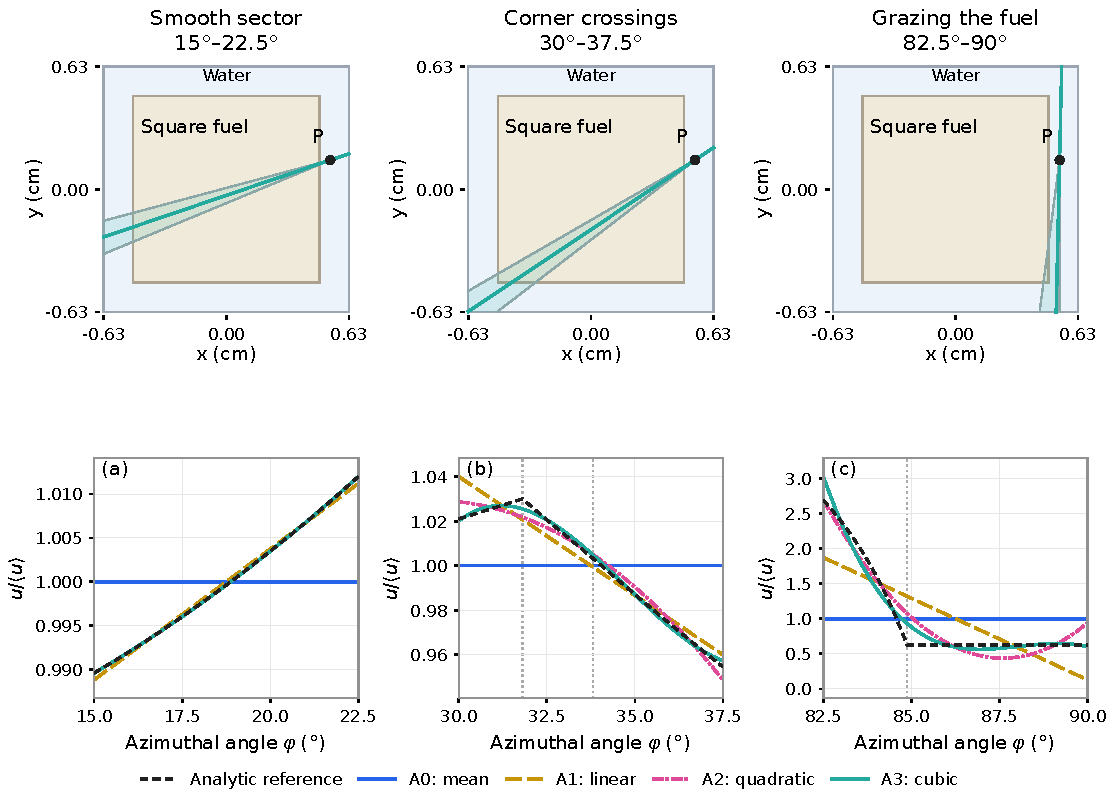
\includegraphics[width=0.98\textwidth]{pin_angular_three_sectors_en.pdf}
\caption{Intra-segment angular representation at a water-region
observation point of a synthetic, purely absorbing square-pin problem
(pin pitch $1.26$~cm, fuel side $0.9571$~cm, observation point
$(0.535,0.15)$~cm, polar angle $90^{\circ}$; fuel/water
$(\Sigma_t,Q)=(1.2,1)/(0.2,0.04)$, vacuum boundary). Reference: even
parity $u=(F_{\Omega}+F_{-\Omega})/2$ from piecewise-analytic ray
transport, normalised by its own sector mean. Curves: orthogonal
Legendre projections of the \emph{same} reference onto
$A{=}0,1,2,3$ --- i.e.\ what the closure with $A$ degrees of freedom
per segment can represent. Top: geometry, the fan is the full angular
sector, the solid ray the representative direction (a) $15$--$22.5^{\circ}$
(smooth), (b) $30$--$37.5^{\circ}$ (fuel-corner at $31.805^{\circ}$
and outer-boundary corner at $33.803^{\circ}$), (c) $82.5$--$90^{\circ}$
(fuel-grazing at $84.869^{\circ}$). Illustration of angular
representation only; not an eigenvalue or accuracy result.}
\label{fig:pinangular}
\end{figure}

\paragraph{The checkerboard of Ref.~\cite{psn2027} at $A{=}3$.}
The first re-computation of Study II's protocol is the strong/weak
absorber checkerboard of Figure~3 of Ref.~\cite{psn2027}: a $2\times2$
base cell of $1$~cm nodes (all edges reflective), one group, fuel
$\Sigma_t{=}1.5$, $\Sigma_s{=}1.35$, $\nu\Sigma_f{=}0.24$ and absorber
$\Sigma_t{=}1.0$ with $\Sigma_s{=}0.93$ (weak) or $0.30$ (strong). We
uniformly subdivide to $2S\times2S$ nodes and sweep
$S{=}1\ldots20$ against $M{=}2,4,8,12,16,24$ --- 240 points per angular
model --- with the $A{=}3$ closure and a $10^{-7}$ convergence gate. The
polar partition is the generic even set with $I{=}30$ segments (15
independent sectors); the source paper's three-polar protocol
was swept as well ($S{=}1\ldots12$). References: the OpenMC values of
the source paper, $1.12974$ (weak) and $0.51673$ (strong), quoted to
five decimals ($\approx\pm0.5$~pcm precision limit).

Figure~\ref{fig:cbA3} gives the $I{=}30$ sweep. Four readings.
(i)~The coarse-grid part converges as second order in the node size:
$S{=}1\to6$ reduces $|\Delta k|$ by a factor $\sim$28 at $M{=}24$
on both absorbers (weak $+458.6\to+16.1$, strong
$+2430.4\to+89.5$~pcm), and the $M$-columns flatten from $M{=}8$ on
--- the angular-segment count is not the bottleneck once the segment
count is above 8.
(ii)~The best point of the whole sweep is the weak absorber at
$S{=}12$, $M{=}16/24$: $-0.1$~pcm, i.e.\ at the precision limit of the
five-decimal reference; on the strong absorber the best point is
$S{=}14$, $M{=}24$ ($-0.5$~pcm) / $S{=}13$, $M{=}8$ ($-1.9$~pcm).
(iii)~Beyond $S{\approx}12$ the deviation from the reference stops
decreasing, and the fine-grid rows settle near a small residual within
this scan: over $S{=}10\ldots20$
each $M{=}24$ column is fit by $b+c_2/S^2$ to $0.02$~pcm RMS (weak)
and $0.08$~pcm RMS (strong), whereas the one-term $b+c_1/S$ form fits
the same data at $0.16$/$0.84$~pcm RMS (the fit uses the unrounded
sweep values) --- roughly a factor of $9$
(weak) to $10$ (strong) worse, i.e.\ the decay is second-order-like
rather than linear. The finite-range data are thus consistent with a
spatial contribution decaying as $S^{-2}$ plus a residual that
persists at the fixed angular discretization --- a reading of a finite
scan, not a proven asymptotic error decomposition; the polar-set
comparison below ($I{=}60$ moves the $S{=}20$ point by $+2.9$~pcm
weak, $+15.3$~pcm strong) shows that residual responds to the polar
partition, but does not by itself establish $I{=}60$ as converged.
Within this scan the points closest to the reference sit at
$S{=}12$--$14$; beyond that range a larger $S$ adds cost without
further reducing the deviation from the reference.
(iv)~The $M{=}2$ column's negative bias deepens with $S$ (weak
$-51.8$, strong $-259.5$ at $S{=}20$): the two-segment azimuthal
representation carries a structural streaming error that refinement
exposes rather than hides.

\begin{figure}[H]
\centering
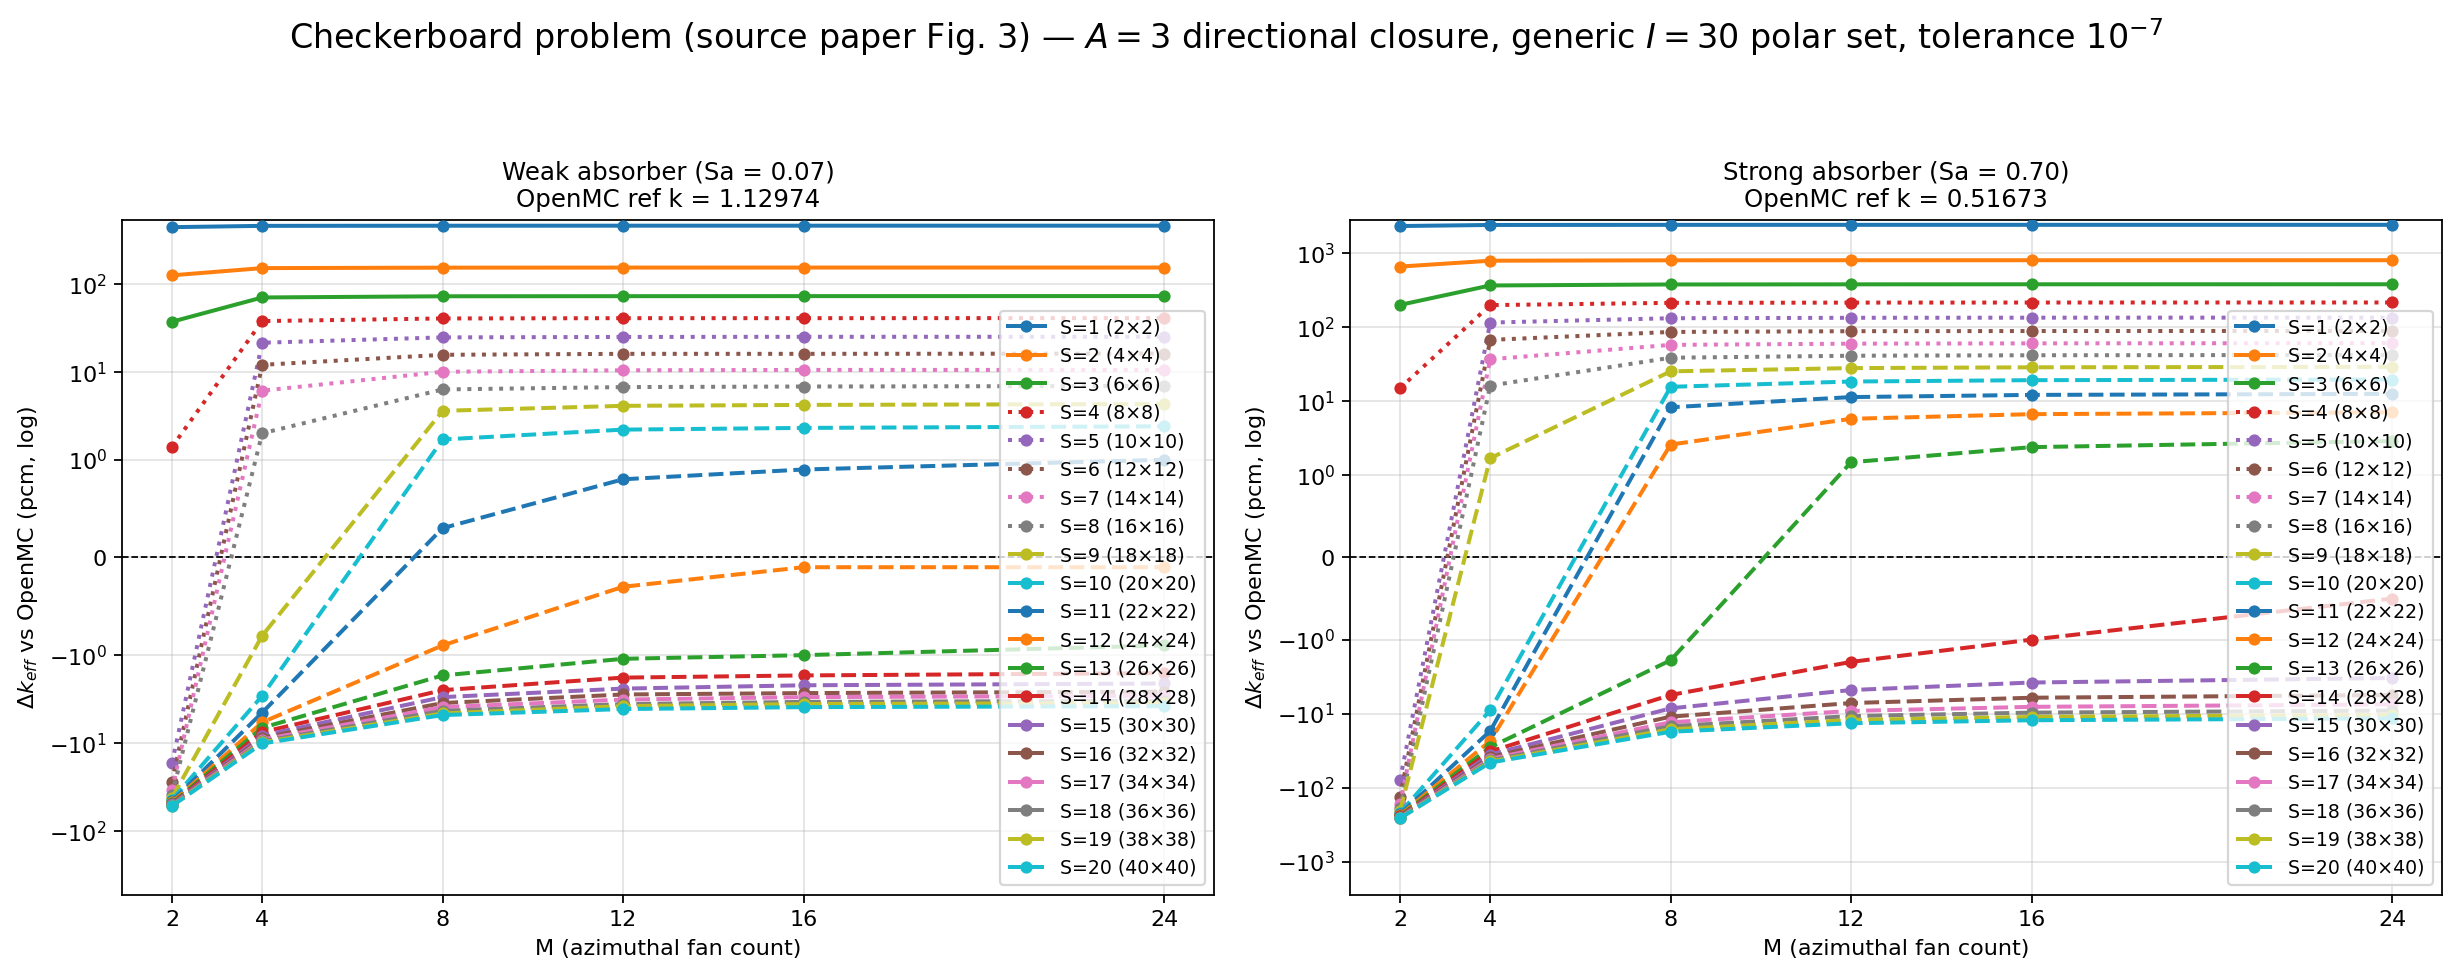
\includegraphics[width=0.98\textwidth]{checkerboard_a3_i30_sm.png}
\caption{Checkerboard of Ref.~\cite{psn2027} Fig.~3, $A{=}3$ closure,
generic $I{=}30$ polar set: $\Delta k$ versus $M$ for each
$S$ ($S{=}1\ldots20$, one curve per subdivision), weak absorber
(left) and strong absorber (right). Vertical axis in symlog: the apparent ``jump'' of the curves
as they cross $\Delta k=0$ is an axis artefact of
$|\Delta k|<1$~pcm being drawn on the linear branch of the symlog
scale --- the underlying data are continuous. All 240 points converged
to $10^{-7}$; best points: weak $S{=}12$, $M{=}16/24$ ($-0.1$~pcm),
strong $S{=}14$, $M{=}24$ ($-0.5$~pcm).}
\label{fig:cbA3}
\end{figure}

Two effects are visible in the fine-grid rows and worth isolating.
First, the signed-error crossing of zero between the coarse-grid
positive bias and the fine-grid offset (e.g.\ weak $S{=}11$--$14$ at
$M{=}16/24$) is consistent with cancellation between a decaying
spatial contribution and a finite-angular-discretization offset:
repeating the $I{=}30$ point at $S{=}20$, $M{=}24$, $A{=}3$
with the even polar set doubled to $I{=}60$ moves the weak-absorber
value from $-3.8$ to $-0.9$~pcm and the strong-absorber value from
$-11.6$ to $+3.7$~pcm. That comparison demonstrates polar-sector
sensitivity; it does not establish a loss of second-order spatial
convergence. The two polar sets do not by themselves prove the
$I{=}60$ residual is converged, nor do they, on the same finite-range
data, separate a polar-quadrature offset from any residual
spatial-basis contribution --- they show the fine-grid residual
responds to the polar partition, and no more. Second, the polar
partition also explains the
coarse/fine gap between the two protocols: on the source paper's
three-polar protocol the same fine-grid points sit at $+3.9$ (weak)
and $+28.6$ (strong)~pcm at $S{=}12$, $M{=}24$, versus $-0.1$ and
$+7.1$~pcm with $I{=}30$ --- the extra polar sectors pay off only
on the finer meshes, where the sensitivity to the polar discretisation
is more visible than the spatial contribution; at $S{=}1$ the two polar
sets agree to within a few pcm.

\paragraph{The $2\times2$ fuel-split tiling.}
The $A{=}3$ closure is run on the C5G7 pin cell with the fuel square
split $2\times2$: each pin cell becomes a
$4\times4$ block of rectangles --- four fuel sub-nodes of side
$s/2{=}0.4786$~cm and a water ring of corner blocks ($0.1514^2$~cm$^2$)
and edge strips ($0.4786\times0.1514$~cm, aspect $3.2{:}1$) ---
Figure~\ref{fig:rect4layout}. The $17\times17$ assembly is
$68\times68{=}4624$ rectangles and the 1/4 core $204\times204{=}41616$;
pin positions, fuel
area and total area are unchanged. The $2\times2$ split is the
tiling in which the edge water strips --- the channels
that carry streaming across the pin --- carry a tangential extent of
$s/2$ (aspect $3.2{:}1$), halved from $s$ (aspect $6.3{:}1$) in the
$3\times3$ tiling, while remaining dedicated water nodes on the
fuel/water interface as they already were. It is the
tiling the $A{=}3$ closure is run on: the angular correction and the
intra-node spatial split act on different parts of the error, and the
$S$ sub-division of Section~2.2 remains available on top of it.

\begin{figure}[H]
\centering
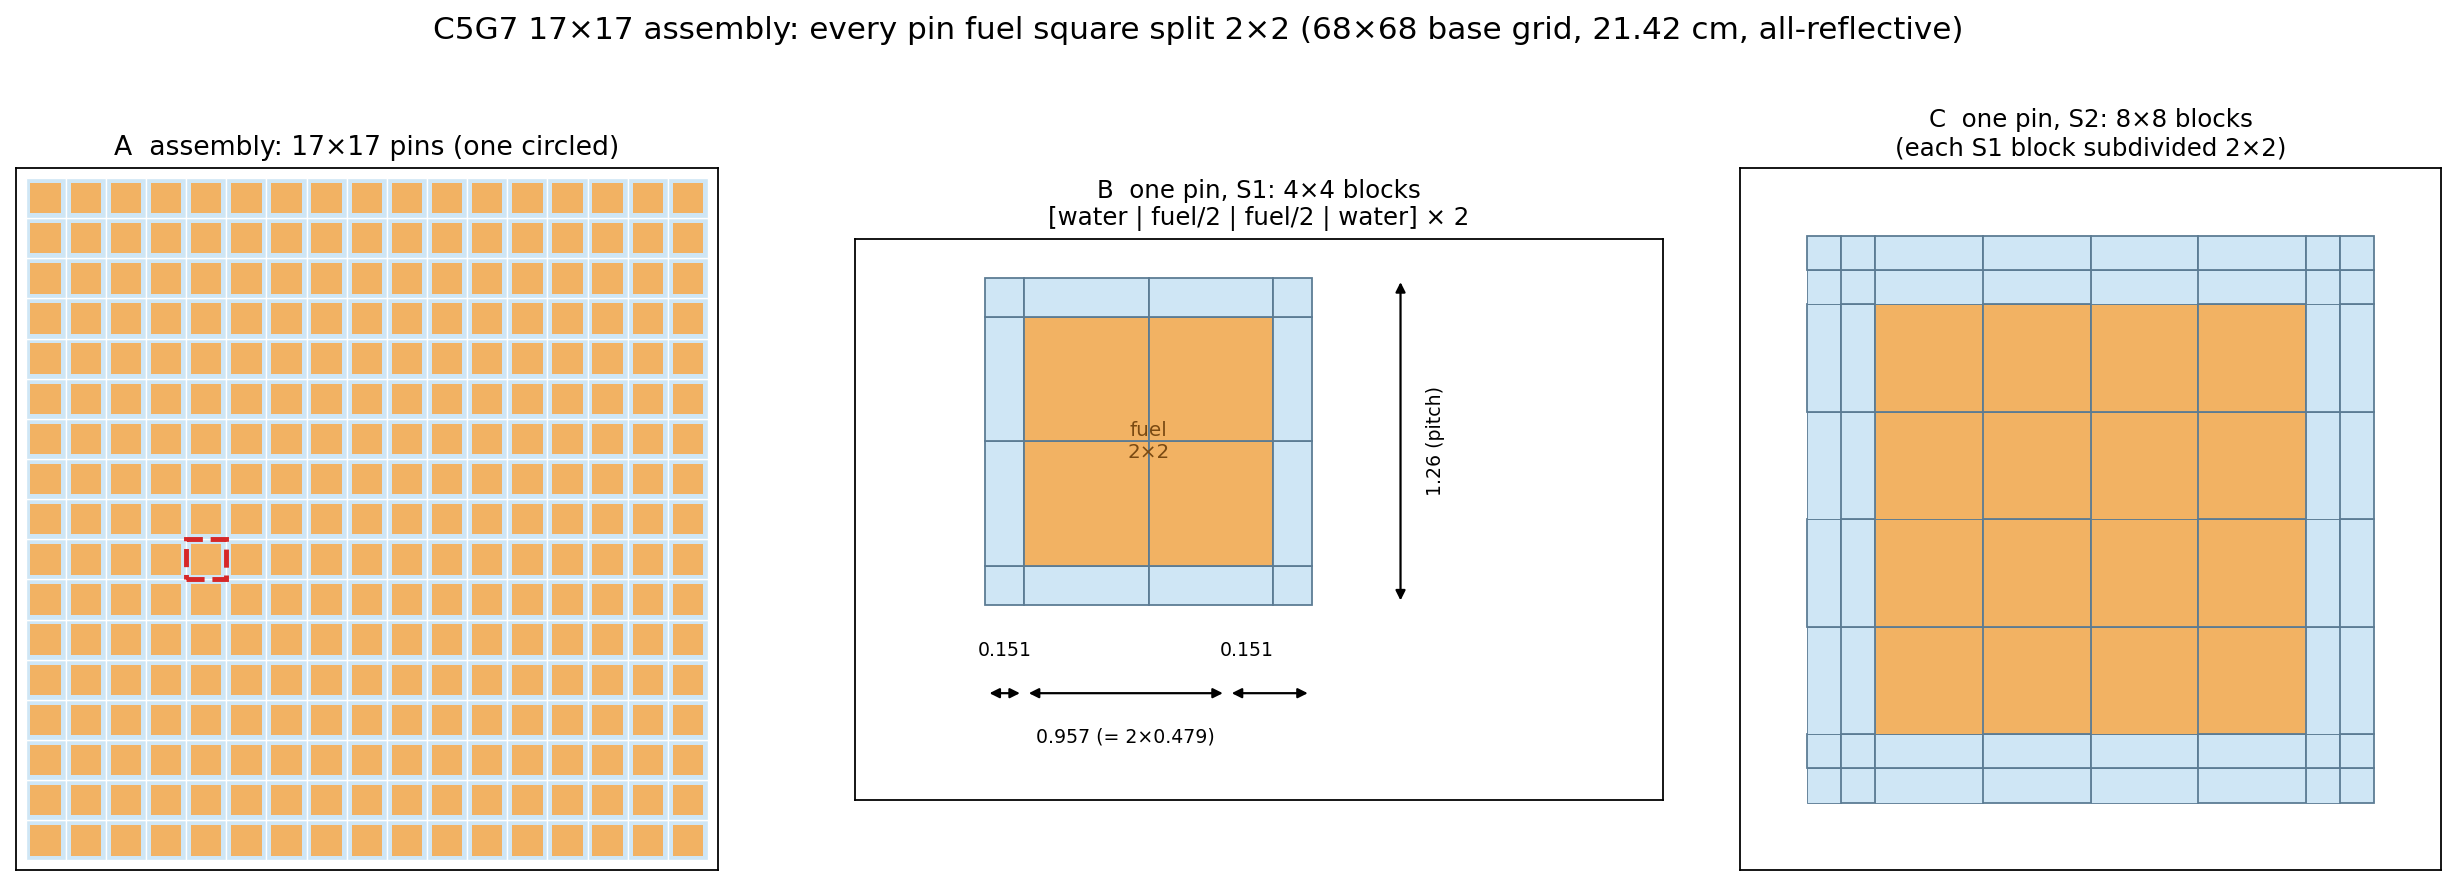
\includegraphics[width=0.98\textwidth]{rect4_pin_geometry.png}
\caption{The $2\times2$ fuel-split tiling of the C5G7 pin
cell. (a) $17\times17$ assembly, one pin circled. (b) One pin at
$S{=}1$: $4\times4$ blocks $[$water $|$ fuel$/2$ $|$ fuel$/2$
$|$ water$]\times2$; water gap $0.1514$~cm, fuel square
$0.957$~cm ($=2\times0.479$). (c) The same pin at $S{=}2$: $8\times8$
blocks.}
\label{fig:rect4layout}
\end{figure}

\paragraph{C5G7 at $A{=}3$: assemblies and core.}
Figure~\ref{fig:a3mconv} gives the $A{=}3$ sweep on the two
$17\times17$ assemblies, $S{=}1,2$ against $M{=}2,4,8,12,16,24$
(24 points, every point converged to $10^{-7}$), and the $S{=}1$ row
of the 1/4-core sweep on the same tiling, against the same-geometry
pure-XS OpenMC references ($1.3347260$ UO$_2$, $1.1851053$ MOX,
$1.1872176$ core; each $\approx\pm3.3$--$3.6$~pcm). The contrast with
the old closure of Study II is direct, but with a caveat: the old
closure ran on the $3\times3$ tiling, where the MOX assembly sat at
$-98.9$~pcm ($S{=}1$, $M{=}24$) and $-33.5$~pcm at its best, while the
$A{=}3$ closure runs on the $2\times2$ fuel-split tiling, where it
sits at $-0.9$~pcm at $M{=}12$, $S{=}1$, inside the Monte
Carlo standard error; on the $S{=}2$ row the same tiling sits at
$-9.8$~pcm at $M{=}24$. The two tilings are not the same mesh
($4624$ vs $2601$ rectangles per assembly at $S{=}1$), so this
contrast measures the new setting --- finer fuel split together with
the $A{=}3$ angular closure --- as a whole rather than the angular
order in isolation. On the
UO$_2$ assembly the best point is $-0.5$~pcm ($S{=}2$, $M{=}24$) and
$-2.8$~pcm on the $S{=}1$ row ($M{=}8$), both inside the
$\pm3.6$~pcm reference uncertainty; the $M$-convergence is monotonic in
signed $\Delta k$ from $M{=}2$ onward on both assemblies; with only
$S{=}1,2$ computed, this scan does not rule out a $S{\ge}3$
non-monotonicity of the Study-II type. The 1/4
core shows the same fast angular convergence on its
$S{=}1$ row --- $-135.6$, $-34.2$ and $-1.7$~pcm at $M{=}2$, $4$, $8$
--- the core reaches the Monte Carlo standard error at $M{=}8$, where
the assemblies need $M{=}12$--$24$; the row then overshoots mildly
($+6.2$~pcm at $M{=}12$, $+9.1$~pcm at $M{=}16$ and $+11.0$~pcm at
$M{=}24$). The whole $S{=}2$ row is in progress.

\begin{figure}[H]
\centering
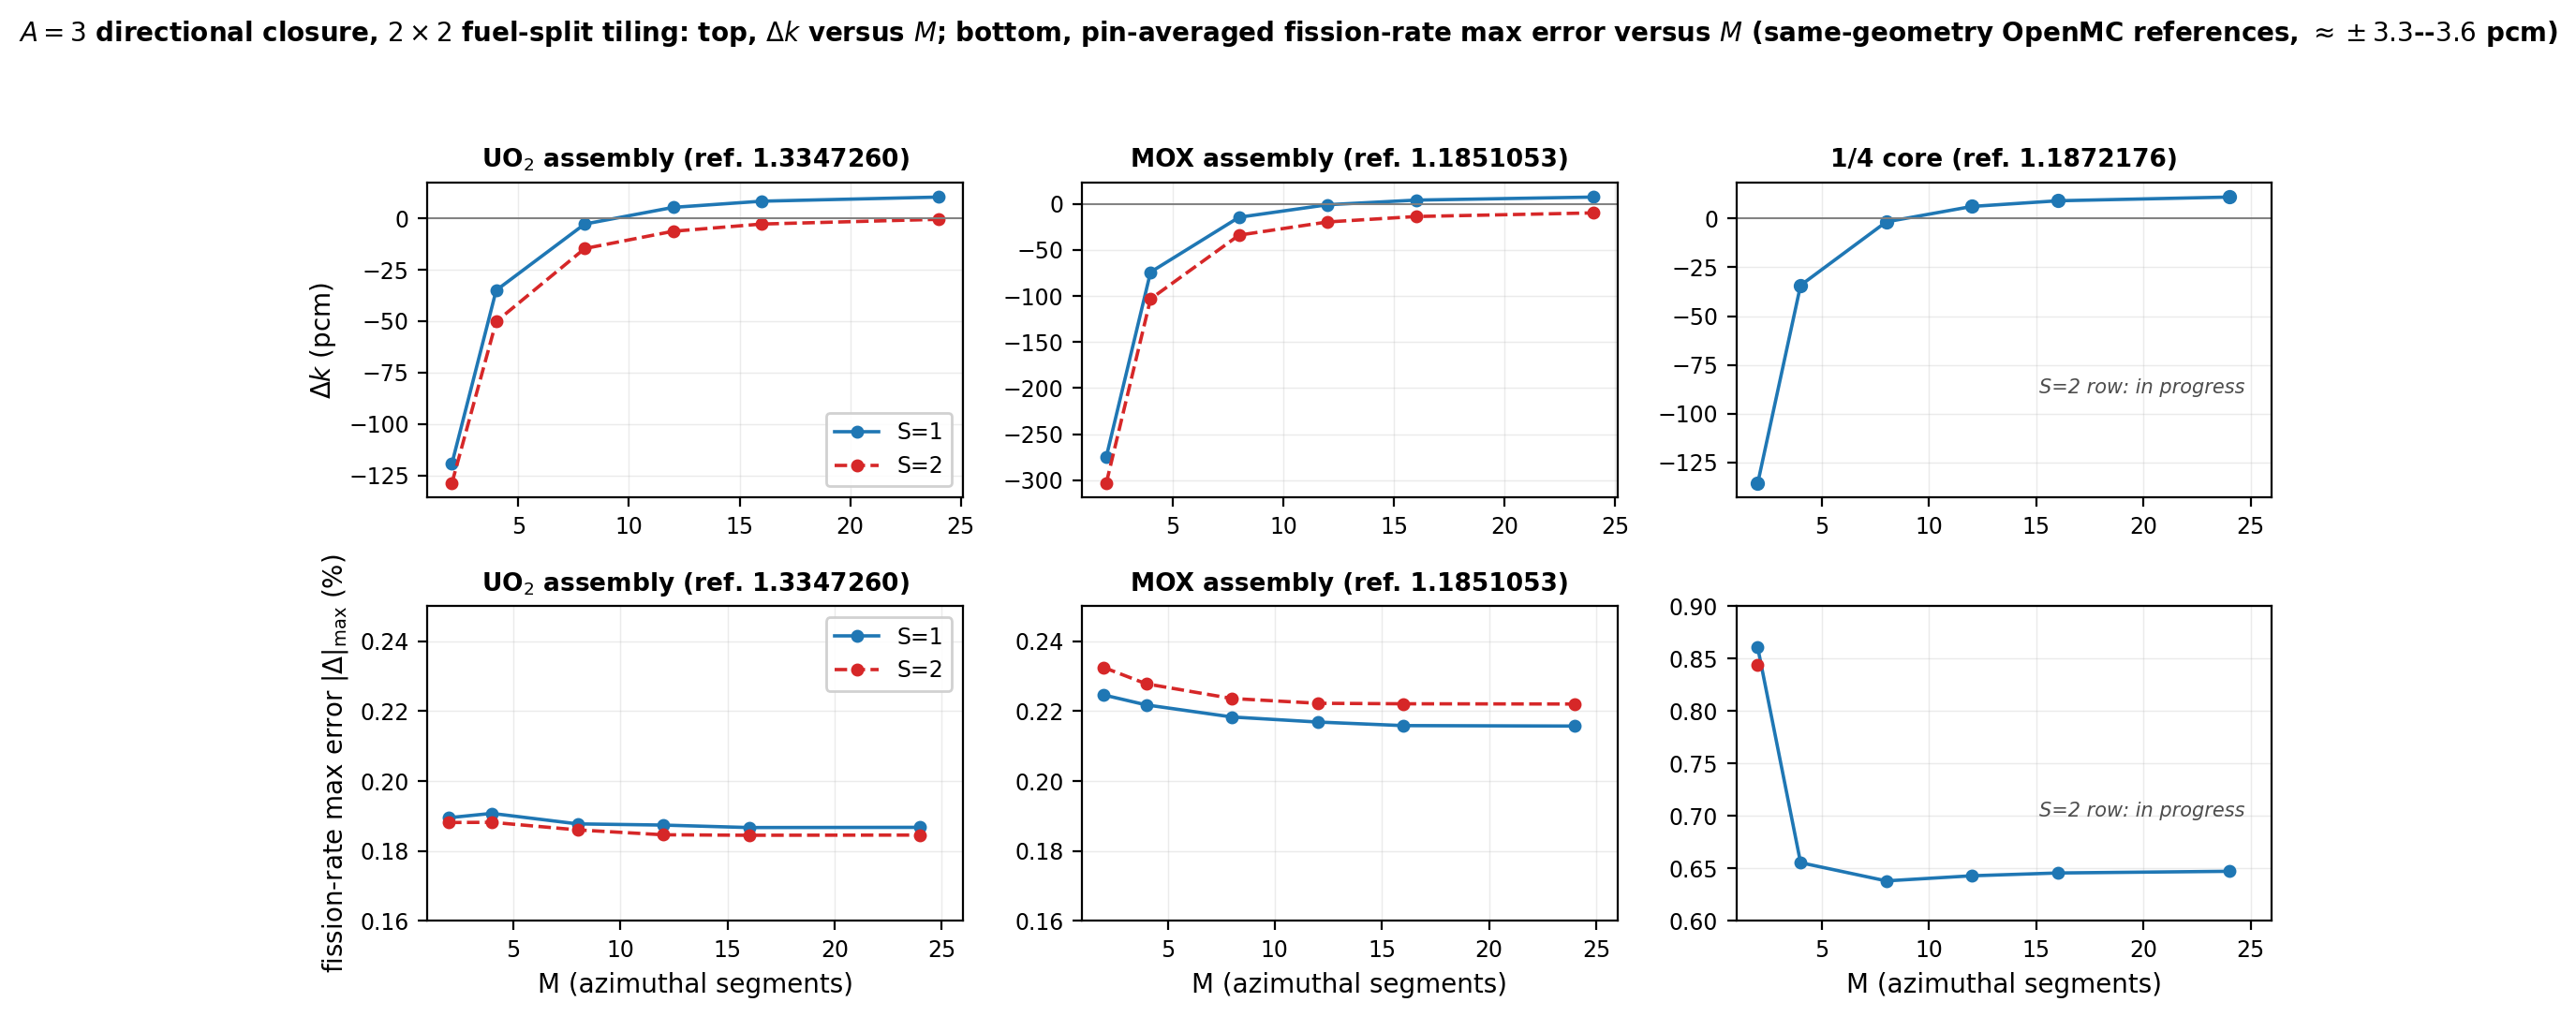
\includegraphics[width=0.98\textwidth]{c5g7_rect4_a3_m_conv.png}
\caption{$A{=}3$ closure, $2\times2$ fuel-split tiling. Top:
$\Delta k$ versus $M$ for $S{=}1,2$ on the UO$_2$ and MOX $17\times17$
assemblies (all 24 points converged to $10^{-7}$) and the completed
$S{=}1$ row of the 1/4 core ($204\times204$ grid; the $S{=}2$ row is in
progress). Bottom:
pin-averaged fission-rate $\Sigma_f\phi$ maximum relative error
(percent) versus $M$, against the same-geometry pure-XS OpenMC
reference power maps, fuel pins only ($264$ assembly pins; core rows
cropped to the $2\times2$ fuel block, $1056$ pins). Same-geometry
references $1.3347260$ / $1.1851053$ / $1.1872176$ (each
$\approx\pm3.3$--$3.6$~pcm). Best points: UO$_2$ $S{=}2$,
$M{=}24$ ($-0.5$~pcm), MOX $S{=}1$, $M{=}12$ ($-0.9$~pcm), core
$S{=}1$, $M{=}8$ ($-1.7$~pcm, best core point).}
\label{fig:a3mconv}
\end{figure}

\paragraph{Fission fields.}
Figure~\ref{fig:a3fission} compares the pin-averaged fission
distributions against the OpenMC reference on the identical geometry:
the pin-by-pin relative error on the 264 fuel pins is $0.055\%$ RMS
(max $0.19\%$) on the UO$_2$ assembly ($\Delta k=-0.5$~pcm, $S{=}2$,
$M{=}24$) and $0.075\%$ RMS (max $0.22\%$) on the MOX assembly
($\Delta k=-9.8$~pcm) --- the field is reference-grade on both
materials at assembly size. On the 1/4 core at $S{=}1$, $M{=}8$
($\Delta k=-1.7$~pcm) the error over all 1056 fuel pins of the
$2\times2$ fuel block is $0.286\%$ RMS (max $0.64\%$).

\begin{figure}[H]
\centering
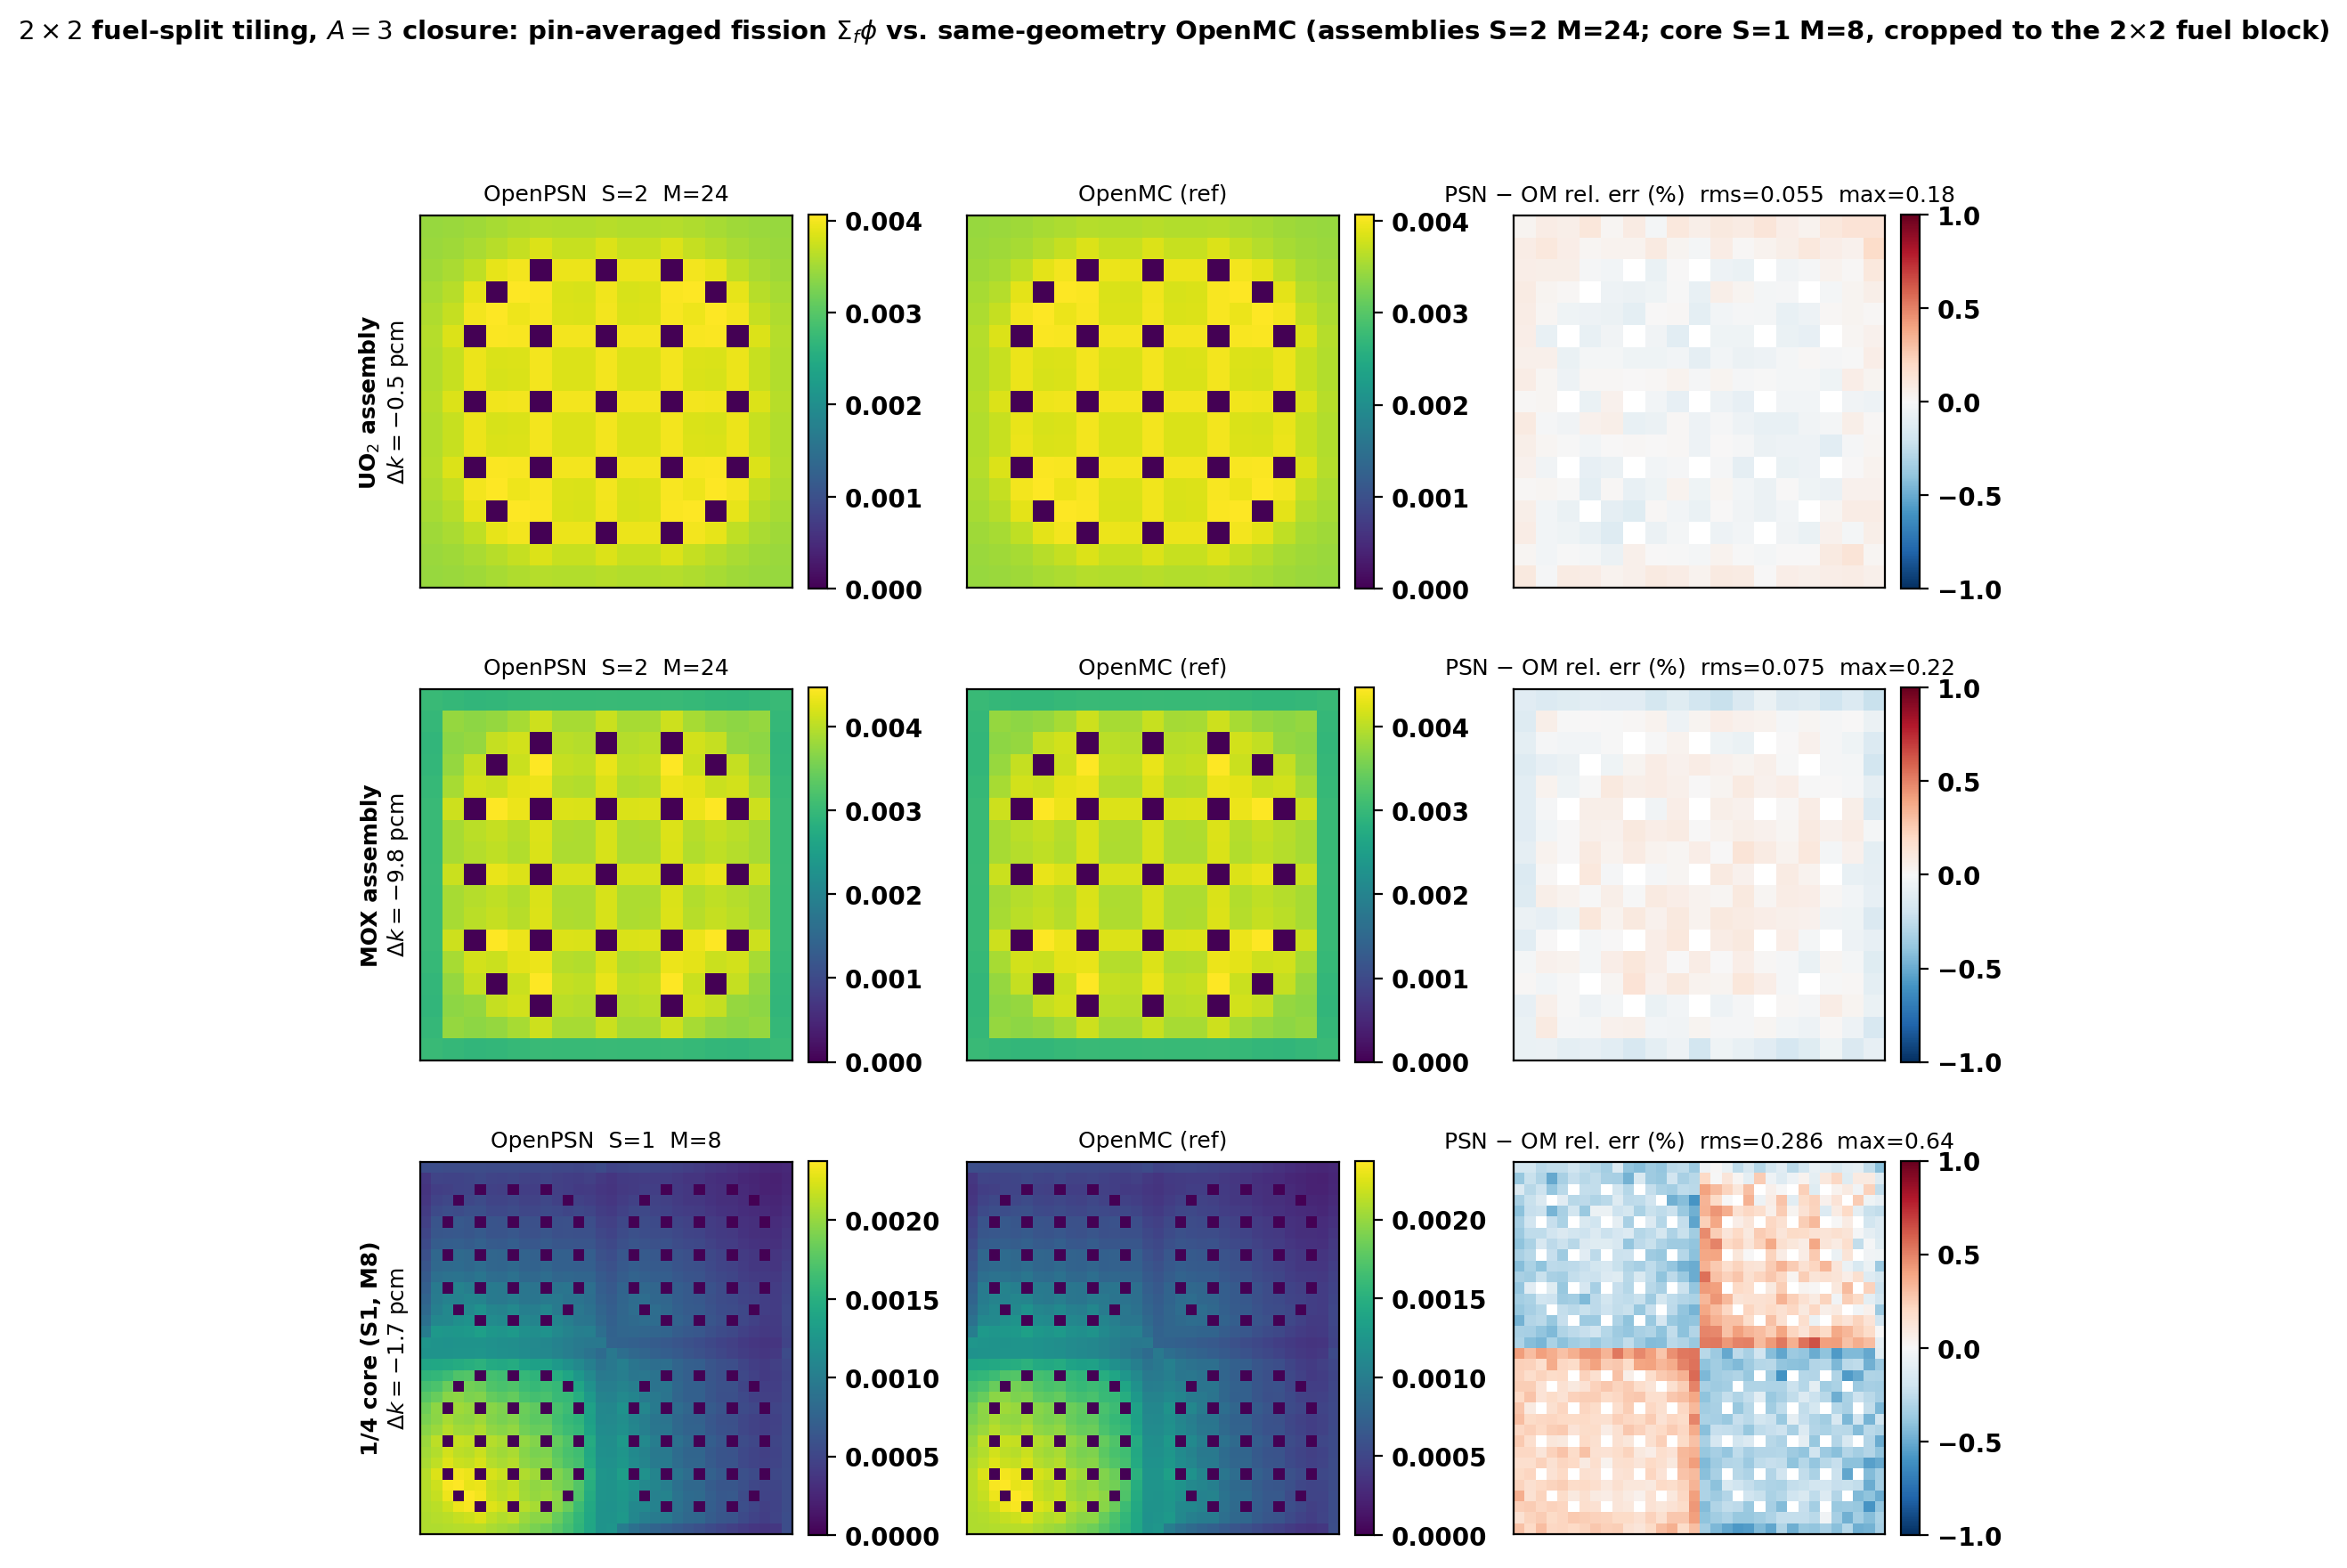
\includegraphics[width=0.98\textwidth]{c5g7_rect4_a3_fission.png}
\caption{$A{=}3$ closure, $2\times2$ fuel-split tiling: pin-averaged fission
$\Sigma_f\phi$, OpenPSN (left), OpenMC on the identical rectangular-rod
geometry (centre), pin-by-pin relative error on fuel pins (right; both
maps normalised to unit sum). Top: UO$_2$ assembly, $S{=}2$, $M{=}24$,
$\Delta k=-0.5$~pcm, RMS $0.055\%$ (max $0.19\%$). Middle: MOX
assembly, $S{=}2$, $M{=}24$, $\Delta k=-9.8$~pcm, RMS $0.075\%$
(max $0.22\%$). Bottom: 1/4 core, $S{=}1$, $M{=}8$, $\Delta k=-1.7$
pcm, RMS $0.286\%$ (max $0.64\%$) over all 1056 fuel pins, cropped to
the $2\times2$ fuel block.}
\label{fig:a3fission}
\end{figure}

\paragraph{Fission-rate convergence across the sweep.}
The bottom row of
Figure~\ref{fig:a3mconv} repeats the field comparison of
Figure~\ref{fig:a3fission} for every
computed point of the sweep, with the identical pin-averaged
fission-rate convention ($\Sigma_f\phi$, unit-sum normalised, fuel
pins only). On the assemblies the field error is essentially flat in
$M$ --- $0.053$--$0.057\%$ RMS on UO$_2$ and $0.075$--$0.081\%$ on
MOX --- even though the eigenvalue error moves by more than
$300$~pcm over the same rows: the pin-averaged power shape is
established by $M{=}4$ and finer angular orders move it by at most
$0.007\%$ RMS across the rows; the maximum pin deviation stays within
$0.18$--$0.19\%$ (UO$_2$) and $0.21$--$0.23\%$ (MOX) over the whole
sweep. The 1/4-core field, cropped to the $2\times2$ fuel block as in
Figure~\ref{fig:a3fission}, sits a factor ${\sim}5$ higher
($0.28$--$0.43\%$ RMS, $0.64$--$0.86\%$ max) and decays from
$M{=}2$ to $M{=}8$ before plateauing along the full $S{=}1$ row
($0.638$--$0.647\%$ max from $M{=}8$ to $M{=}24$).
This sweep does not separate
the OpenMC power-tally statistics from the residual method error at
that floor; the numbers are reported as the measured field
agreement, not as a proven limit. The $S{=}2$ core row beyond
$M{=}2$ is still in progress.


\paragraph{Where the method now stands.}
The sequence of this paper is, in retrospect, a sequence of error
sources being identified and removed one by one. The implementation
\emph{reproduces} the published PSN results to a few pcm
(Section~3). The rectangular-node extension \emph{removes the
homogenisation model} and exposes the next error: the $A{=}0$ angular
closure is incomplete for strongly coupled pin geometries (Study II:
non-monotonic $M$ and $S$ convergence, a $-99$~pcm MOX bias at
$M{=}24$ that the $S\times M$ refinement does not drive toward zero). The $A{=}3$ directional closure of
this section --- derived above from the original transport equation
through the exact parity elimination, the segment-resolved angular
moments and the matrix hyperbolic body --- \emph{narrowed the angular
component of the error}: on the published checkerboard, its
coarse-grid error decays close to second order in $S$
($\sim$28-fold from $S{=}1$ to $6$ at
$M{=}24$); the sweep crosses the five-decimal reference within
$0.1$~pcm (weak absorber, $S{\approx}12$) --- a finite-range
crossing, not a proven asymptotic limit --- and the $S{=}20$ point
shifts from $-3.8$ to $-0.9$~pcm when the polar set is doubled to
$I{=}60$,
and on C5G7 the same closure brings the MOX assembly --- the hardest
case of the benchmark --- to $-0.9$~pcm at $M{=}12$ ($S{=}1$), with
$0.055$--$0.075\%$-RMS fission fields at $S{=}2$, $M{=}24$, and the
1/4 core to $-1.7$~pcm at $M{=}8$ ($S{=}1$); on these points the method
sits within the same-geometry OpenMC standard error, although the scans
do not yet establish the limiting accuracy. The result is a
diffusion-based higher-order angular-mode directional PSN algorithm ---
the hyperbolic-plus-source spatial basis, Legendre angular expansion
within each segment, direction-matrix body closure --- on a compact
nodal grid, without a discrete-ordinates or characteristics mesh.
